This study investigates the potential of combining static analysis tools with \aclp{llm} to enhance the detection of software vulnerabilities while addressing the issue of false positives. 
The methodology involves using two static analyzers, CodeQL and Infer, to flag vulnerabilities, enriching their output with additional code context obtained through a code graph of the project, and leveraging an \ac{llm} to refine the results. 
Figure~\ref{workflow} provides an overview of the workflow.

\begin{figure}[H]
    \centering
    \resizebox{\textwidth}{!}{%
        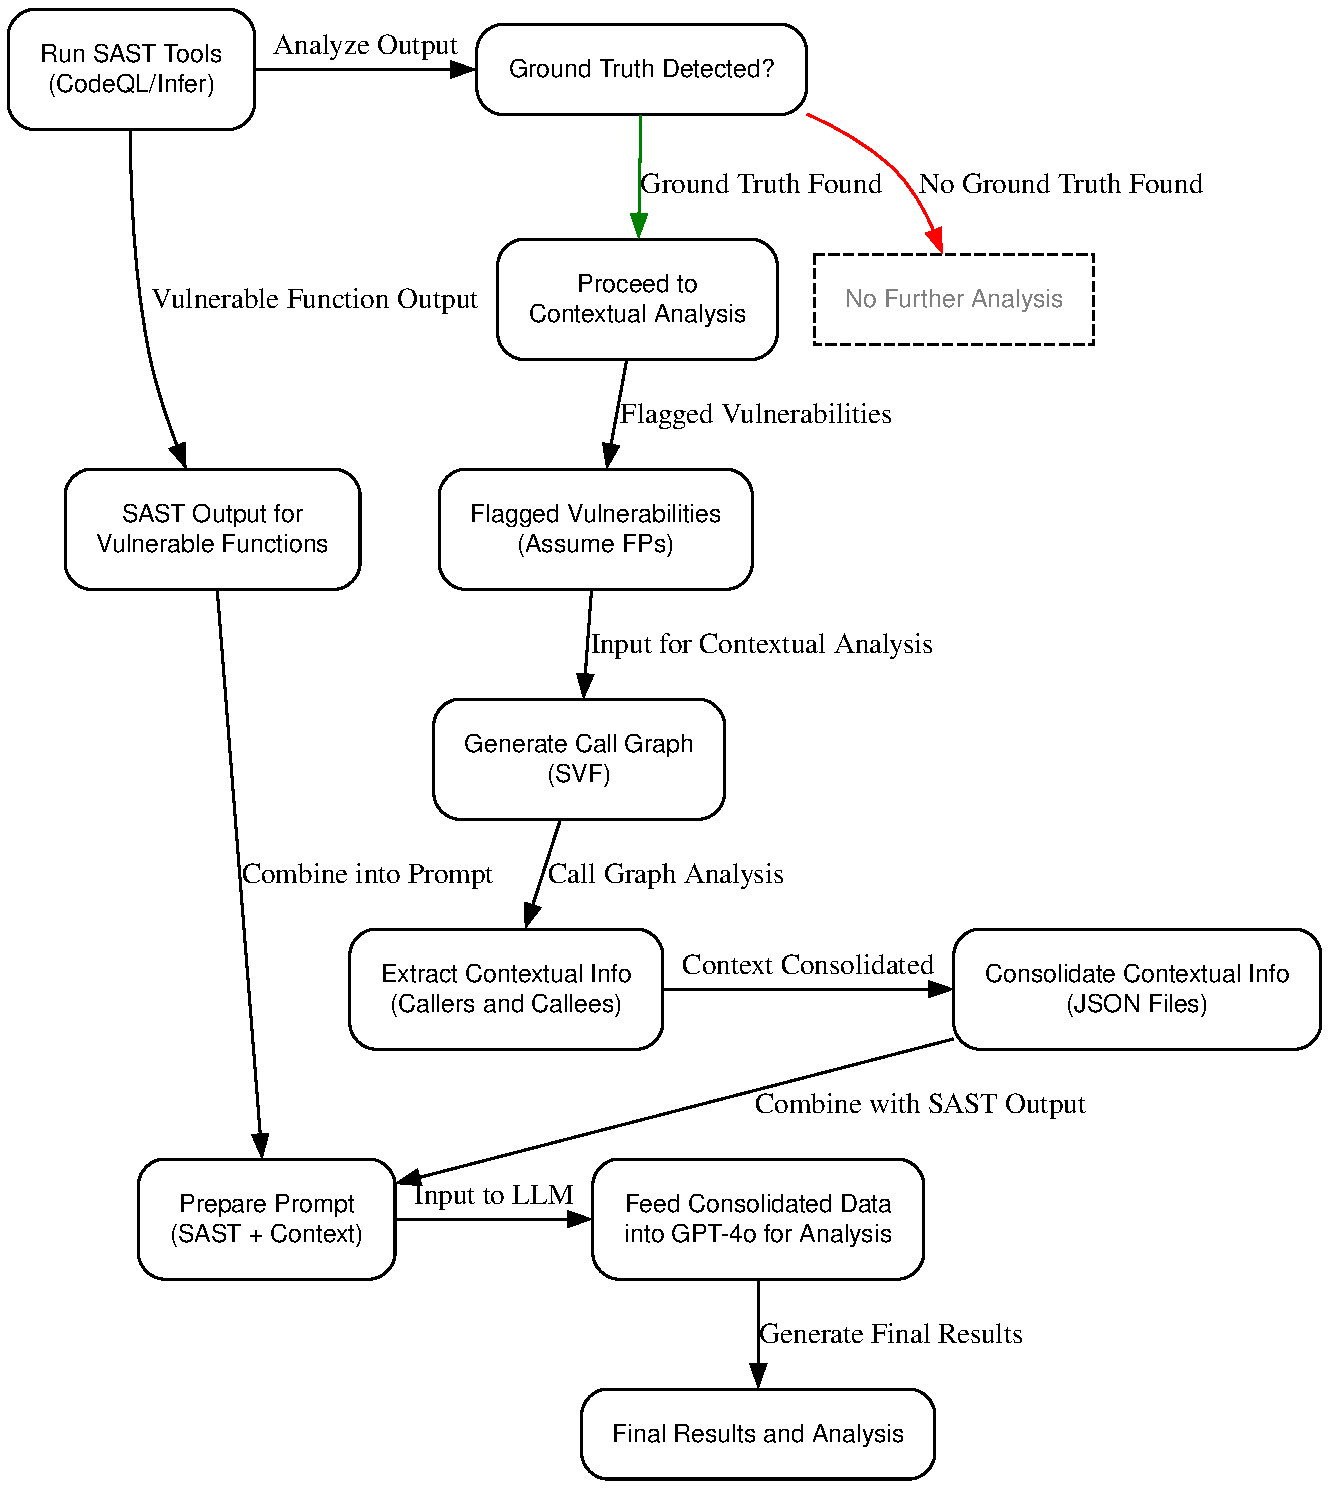
\includegraphics{figures/workflow.pdf} % Path to your diagram file
    }
    \caption{Overview of the workflow combining SAST tools, contextual analysis, and LLM augmentation.}
    \label{workflow}
\end{figure}

In each of the following subsections, detailed explanations of the tools used will be provided, with the goal of clarifying the diagram illustrated above step by step.